%!TeX spellcheck = en-GB

%Basics
\documentclass[aps, prb, a4paper, english, 12pt, twocolumn, longbibliography, amsmath, amssymb, colorinlistoftodos, floatfix]{revtex4-1}
\usepackage[utf8]{inputenc}
\usepackage{babel}

%Symbols and scientifics
\usepackage{amsmath, amsfonts, amssymb, bm}
\usepackage{physics}
\usepackage{mathtools}
\usepackage{siunitx}
\sisetup{
	per-mode = power ,
	round-mode = figures ,
	round-precision = 3 ,
	scientific-notation = false ,
	output-decimal-marker = {.} ,
	exponent-product = \times ,
	separate-uncertainty = true ,
	uncertainty-separator = \ ,
	output-product = \cdot ,
	quotient-mode = fraction ,
	range-phrase = - ,
	range-units =  single ,
	inter-unit-product = \ensuremath{{\cdot{}}} ,
	number-unit-product = \ ,
	multi-part-units = single ,
	alsoload = synchem ,
}

%Appendix, TOC and Bibliography
\usepackage{appendix}
\renewcommand\appendixtocname{Appendices}
%\usepackage[nottoc]{tocbibind}
\usepackage[lastpage,user]{zref}

%Figures
\usepackage[svgnames]{xcolor} % Required to specify font color
\usepackage{float}
\usepackage{graphicx}
\usepackage{subcaption}
\usepackage{caption}
\usepackage{wrapfig}
\usepackage[a4paper, centering, rmargin=2.5cm, tmargin=2.5cm, lmargin=2.5cm, bmargin=2.5cm]{geometry}
\usepackage{etoolbox}
\usepackage{verbatim}
\usepackage[space]{grffile}
\usepackage[final]{pdfpages}
\usepackage{array}
\usepackage{multirow}
\usepackage{dcolumn}
%\usepackage{animate}
\usepackage{fontawesome}
\usepackage[european]{circuitikz}
\usepackage{pgfplots}
\pgfplotsset{width=10cm}
\usepgfplotslibrary{external}
\tikzexternalize

%Header footer
\usepackage{fancyhdr}
\pagestyle{fancy}
\lhead{C. V. Sørensen \\ R. K. F. Wiuff}
\chead{Measuring Capacitance\\of Suspended Graphene Devices}
\rhead{July \nth{27}\\2018}
\cfoot{Page \thepage\, of \zpageref{LastPage}}
\renewcommand{\headrulewidth}{0.4pt}
\renewcommand{\footrulewidth}{0.4pt}

%Text tools
\usepackage[super]{nth}
\usepackage[normalem]{ulem}
\usepackage{import}
\usepackage{url}
\usepackage{lipsum}
\usepackage{microtype}
\usepackage{hyperref}
\hypersetup{
	colorlinks   = true, %Colours links instead of ugly boxes
	urlcolor     = blue, %Colour for external hyperlinks
	linkcolor    = blue, %Colour of internal links
	citecolor   = red %Colour of citations
}
\usepackage[capitalise]{cleveref}
\usepackage{enumitem}
\setlist[enumerate]{itemsep=0mm}
\usepackage{booktabs}
\usepackage{silence}
\usepackage{todonotes}
\WarningFilter{revtex4-1}{Repair the float}

%Python
\usepackage{minted}
\setminted{fontsize=\small}
\usemintedstyle{monokai}
\renewcommand{\listoflistingscaption}{Listings}

%Definitions and new commands
\newcommand{\logas}[1]{\log_{_{10}}{\left( #1 \right)}}
\newcommand{\sins}[1]{\sin{\left( #1 \right)}}
\newcommand{\tans}[1]{\tan{\left( #1 \right)}}
\newcommand{\coss}[1]{\cos{\left( #1 \right)}}
\newcommand{\sinas}[1]{\sin{\left( #1 \degr \right)}}
\newcommand{\tanas}[1]{\tan{\left( #1 \degr\right)}}
\newcommand{\cosas}[1]{\cos{\left( #1 \degr\right)}}
\newcommand{\lnas}[1]{\mathrm{ln}\left( #1 \right)}
\newcommand{\degr}{^{\circ}}
\newcommand{\me}{\mathrm{e}}
\newcommand{\eula}[1]{ \dpd{L }{#1} - \dod{}{t}\left(\dpd{L}{\dot{#1}}\right)}

%PDFPages and RevTeX incompatability fix
\makeatletter
\AtBeginDocument{\let\LS@rot\@undefined}
\makeatother

\begin{document}
%Titlepage herunder:
\begin{abstract}
	\begin{description}
		\item[Abstract] Abstract
	\end{description}
\end{abstract}

\title{10401\\Fusion Energy and Plasma Physics}
\date{January \nth{24} 2018}
\author{Rasmus Kronborg Finnemann Wiuff (s163977)}
\email[E-mail at ]{s163977@student.dtu.dk}
\author{Nicklas Kihm (s143286)}
\email[E-mail at ]{spacrone@live.dk}
\affiliation{Technical University of Denmark}
\homepage[Homepage of the Technical University of Denmark ]{http://www.dtu.dk/english/}
%\homepage[\\\faGithub \ Project Code Repository: ]{https://github.com/rwiuff/Nanomechanics-for-graphene-membranes}
\maketitle

\pagenumbering{arabic}

\tableofcontents

% ToC before List-ofs fix
\makeatletter
\let\toc@pre\relax
\let\toc@post\relax
\makeatother

\thispagestyle{empty}
%\newpage
\setcounter{page}{1}

%Text
\section{Intro}
% !TEX root = ../Main.tex
In recent years a large and quickly growing collaboration between plasma physcisists and engineers have materialised into one of the most ambitious energy producing projects ever seen. The proof-of-concept plasma fusion tokamak reactor ITER\footnote{\url{https://www.iter.org/}} in Cadarache is currently taking shape in order to adress the issue of growing energy demands and climate changes.\newline The mission is simple: Prove that plasma fusion is a viable source of electricity.\newline
Whilst not being the most surmountable task, many researchers and institutions have gathered from across the world, including the Department of Physics at DTU.\newline
In this paper, three assignments are solved as part of the course ``10401 Fusion Energy and Fusion Plasma Physics''. Some key aspects of fusion plasma fueled reactors are adressed and discussed in the assignments.

\begin{acknowledgments}
	The authors would like to thank...
\end{acknowledgments}
%End of text

%Bibliography herunder:
\newpage
\onecolumngrid
\bibliography{Bibliography}

\newpage
\listoffigures
\listoftables
\listoflistings
%\listoftodos
\newpage
%Appendicer herunder:
% !TEX root = Main.tex
\appendix
\appendixpage
\addappheadtotoc
\section{tokamakDTU\textunderscore asign\textunderscore 1}\label{tokamakDTU_asign_1}
\inputminted[bgcolor=Black,linenos=true]{matlab}{Listings/tokamakDTU_asign_1.m}\newpage
\section{IterateTokamakDTU}\label{IterateTokamakDTU}
\inputminted[bgcolor=Black,linenos=true]{matlab}{Listings/IterateTokamakDTU.m}\newpage
\section{Iterations over Freidberg's model}\label{ITFR}
\begin{figure}[H]
	\centering
	\begin{subfigure}[h!]{.45\textwidth}
		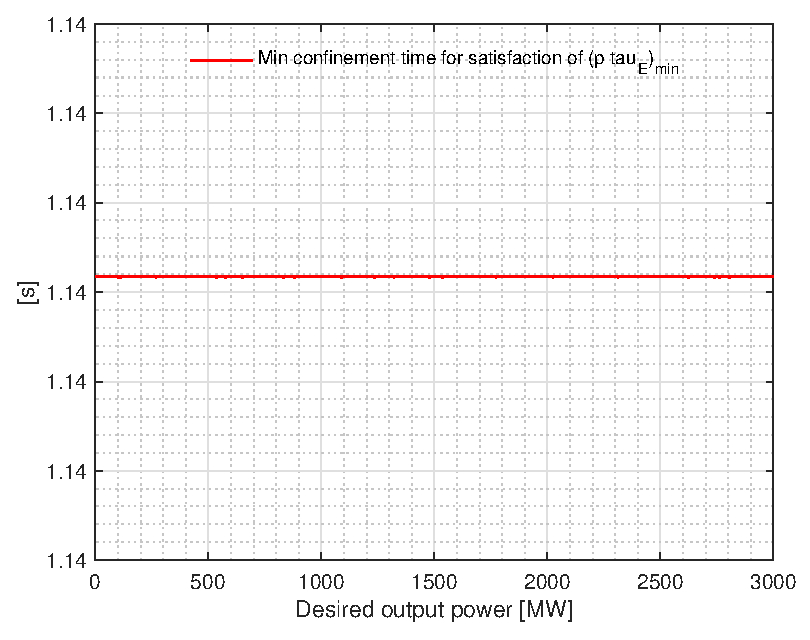
\includegraphics[width=\textwidth]{MatlabFigures/PE/f1.eps}
	\end{subfigure}
	~
	\begin{subfigure}[h!]{.45\textwidth}
		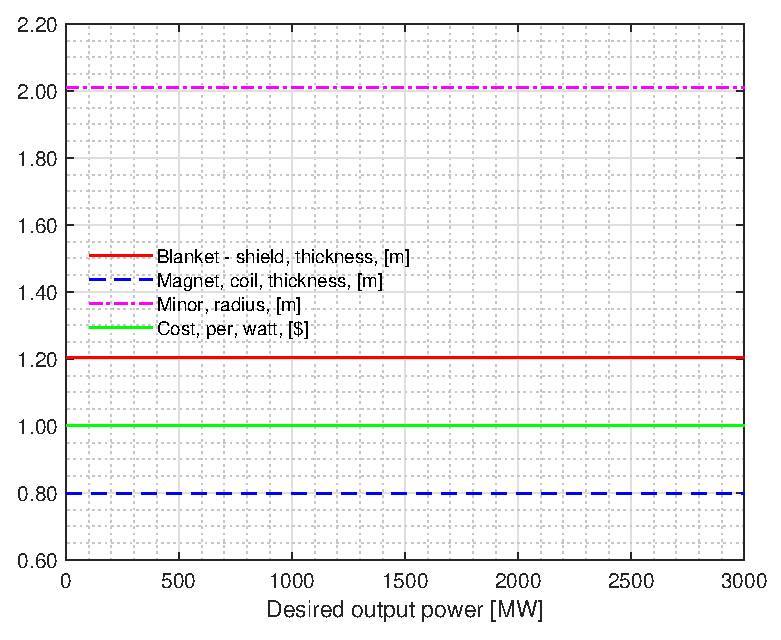
\includegraphics[width=\textwidth]{MatlabFigures/PE/f2.eps}
	\end{subfigure}

	\begin{subfigure}[h!]{.45\textwidth}
		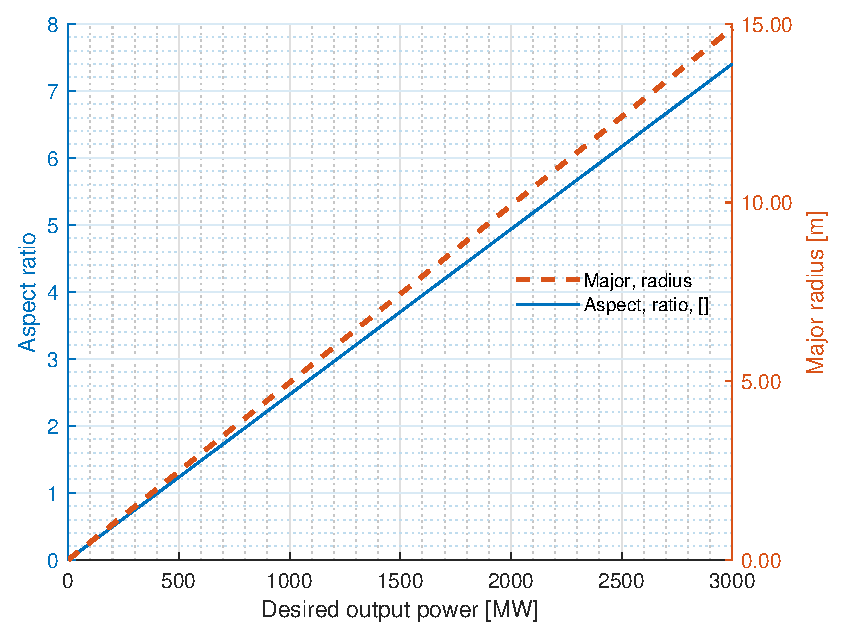
\includegraphics[width=\textwidth]{MatlabFigures/PE/f3.eps}
	\end{subfigure}
	~
	\begin{subfigure}[h!]{.45\textwidth}
		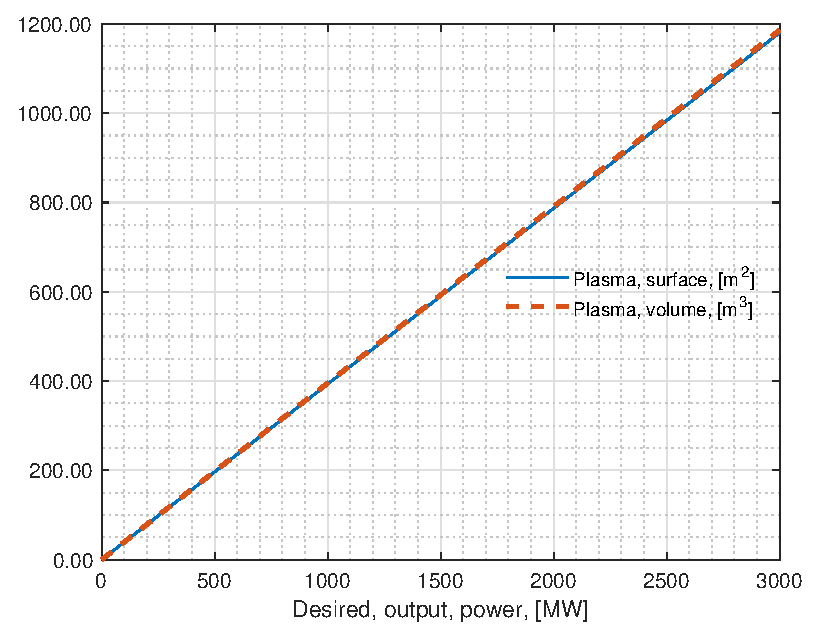
\includegraphics[width=\textwidth]{MatlabFigures/PE/f4.eps}
	\end{subfigure}

	\begin{subfigure}[h!]{.45\textwidth}
		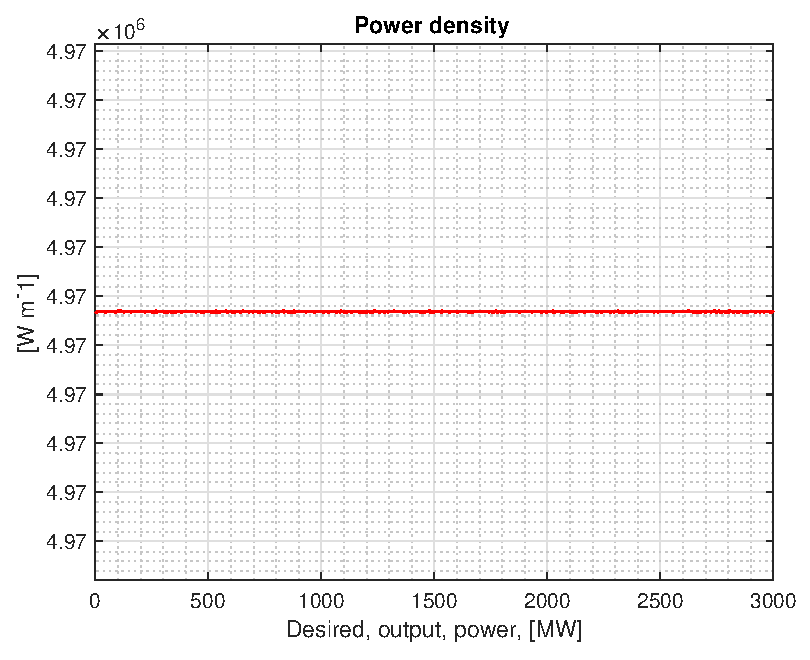
\includegraphics[width=\textwidth]{MatlabFigures/PE/f5.eps}
	\end{subfigure}
	~
	\begin{subfigure}[h!]{.45\textwidth}
		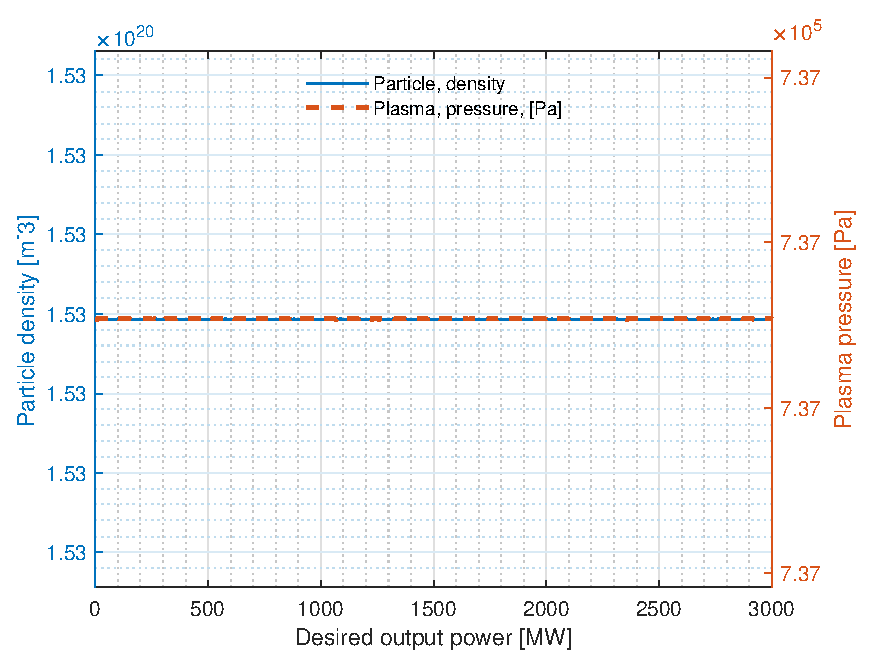
\includegraphics[width=\textwidth]{MatlabFigures/PE/f6.eps}
	\end{subfigure}

	\begin{subfigure}[h!]{.45\textwidth}
		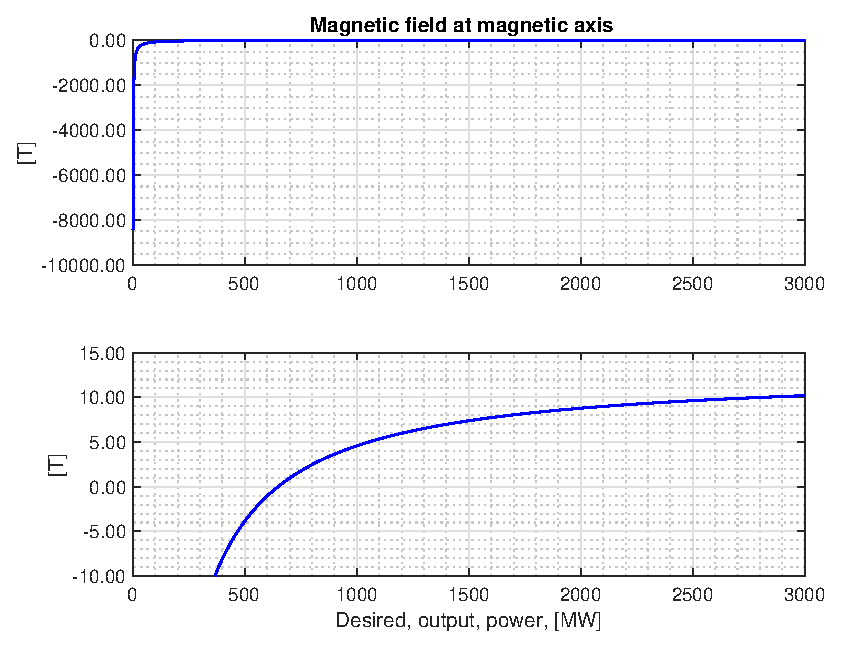
\includegraphics[width=\textwidth]{MatlabFigures/PE/f7.eps}
	\end{subfigure}
	~
	\begin{subfigure}[h!]{.45\textwidth}
		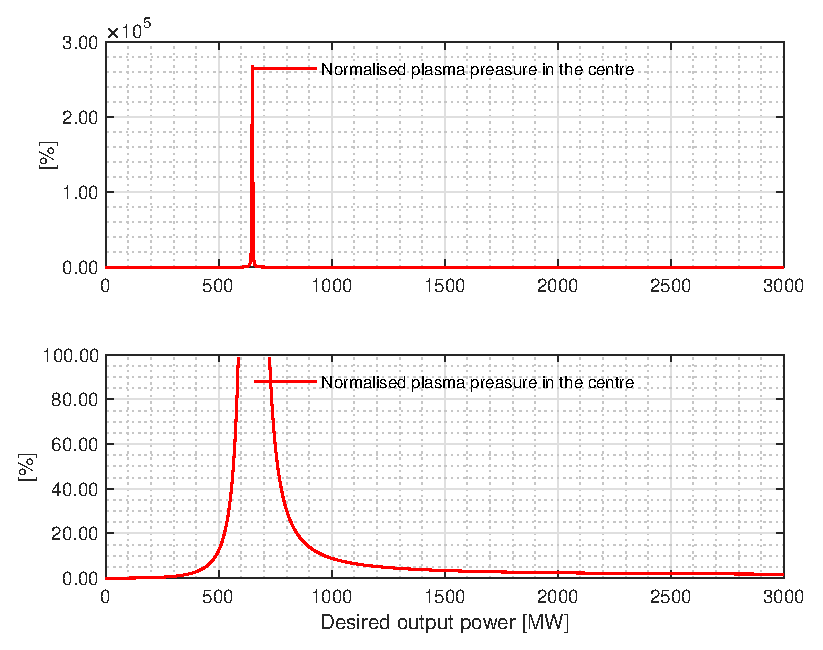
\includegraphics[width=\textwidth]{MatlabFigures/PE/f8.eps}
	\end{subfigure}
\end{figure}
\begin{figure}[H]
	\centering
	\begin{subfigure}[h!]{.45\textwidth}
		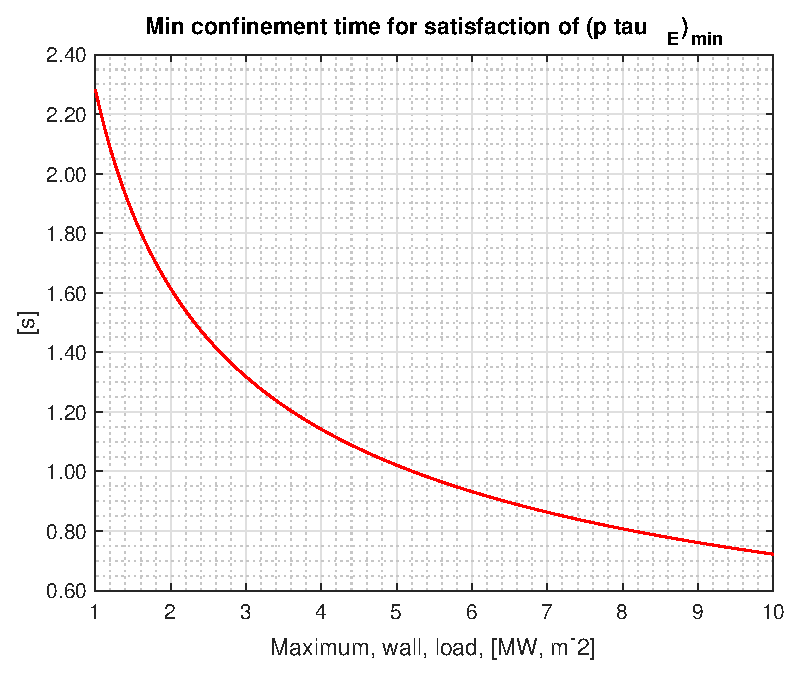
\includegraphics[width=\textwidth]{MatlabFigures/PW/f1.eps}
	\end{subfigure}
	~
	\begin{subfigure}[h!]{.45\textwidth}
		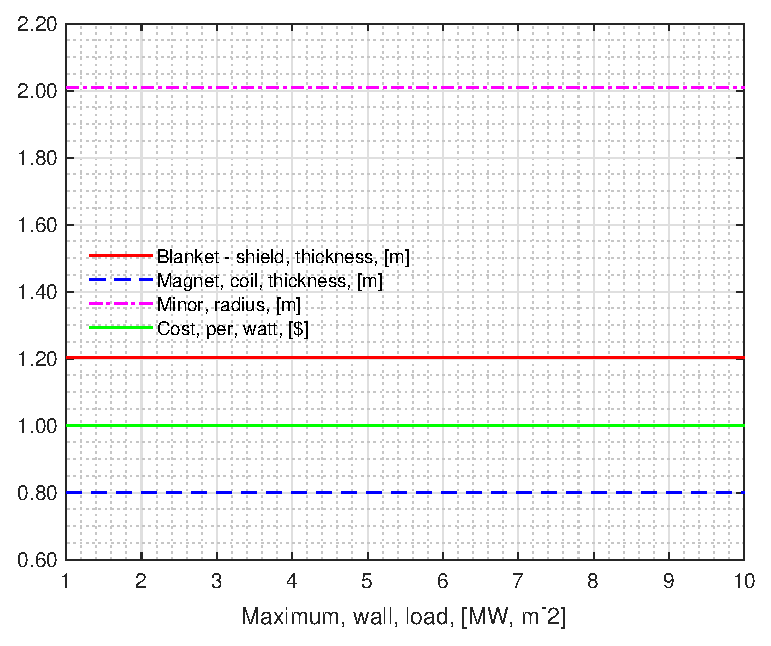
\includegraphics[width=\textwidth]{MatlabFigures/PW/f2.eps}
	\end{subfigure}

	\begin{subfigure}[h!]{.45\textwidth}
		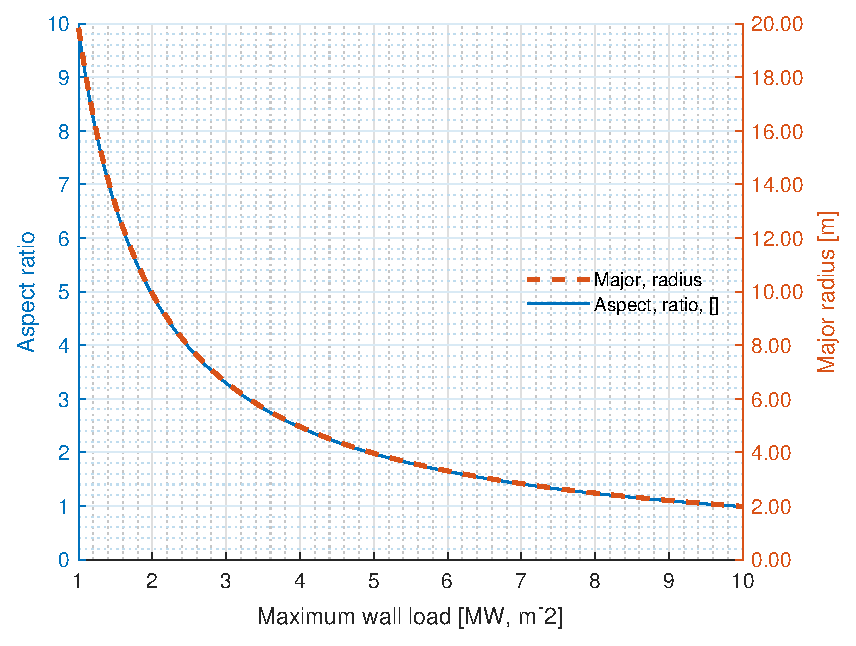
\includegraphics[width=\textwidth]{MatlabFigures/PW/f3.eps}
	\end{subfigure}
	~
	\begin{subfigure}[h!]{.45\textwidth}
		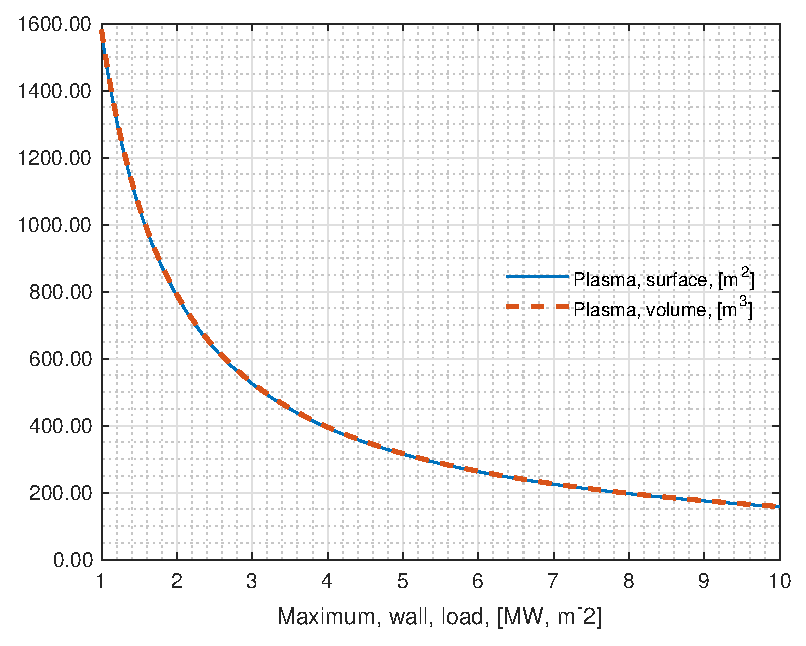
\includegraphics[width=\textwidth]{MatlabFigures/PW/f4.eps}
	\end{subfigure}

	\begin{subfigure}[h!]{.45\textwidth}
		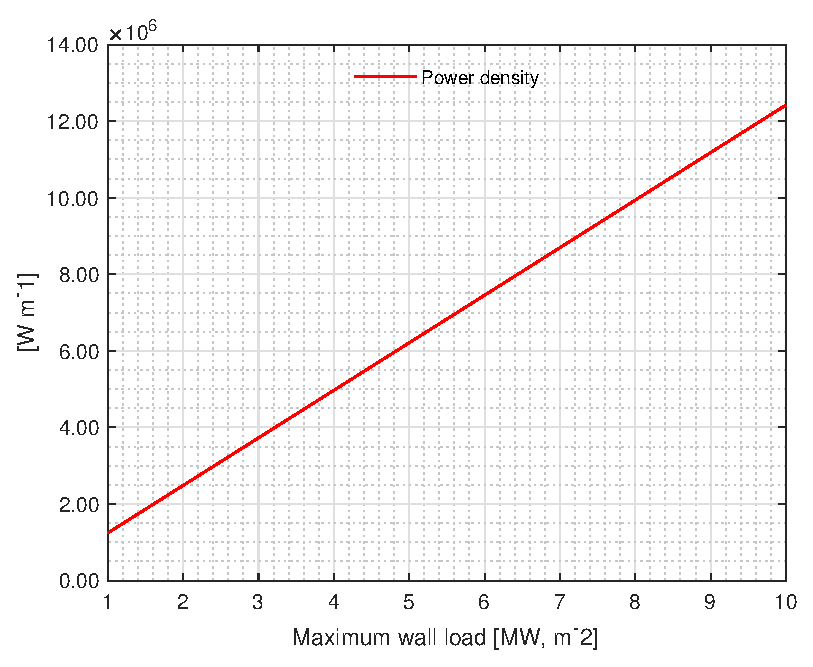
\includegraphics[width=\textwidth]{MatlabFigures/PW/f5.eps}
	\end{subfigure}
	~
	\begin{subfigure}[h!]{.45\textwidth}
		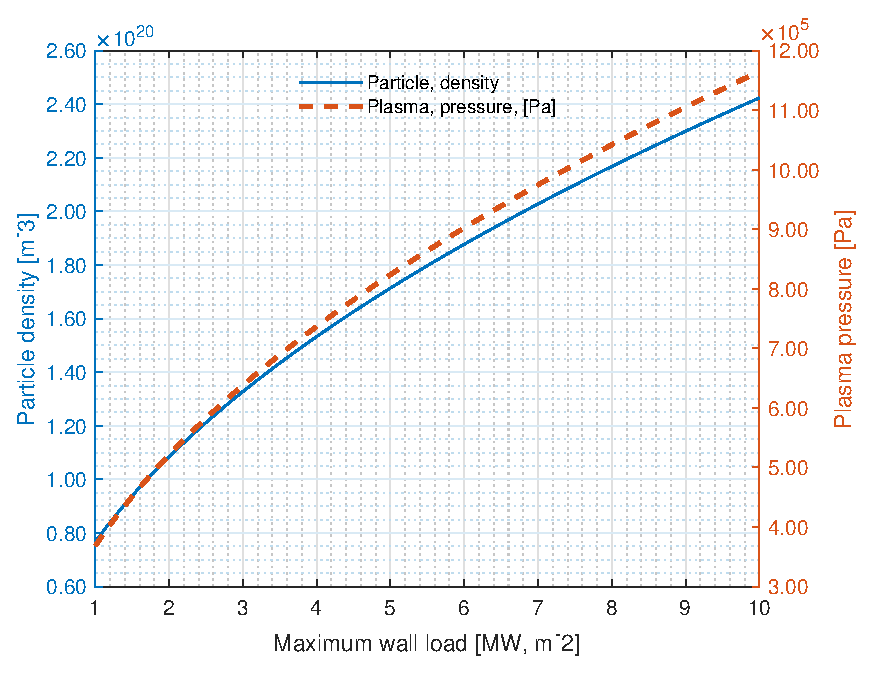
\includegraphics[width=\textwidth]{MatlabFigures/PW/f6.eps}
	\end{subfigure}

	\begin{subfigure}[h!]{.45\textwidth}
		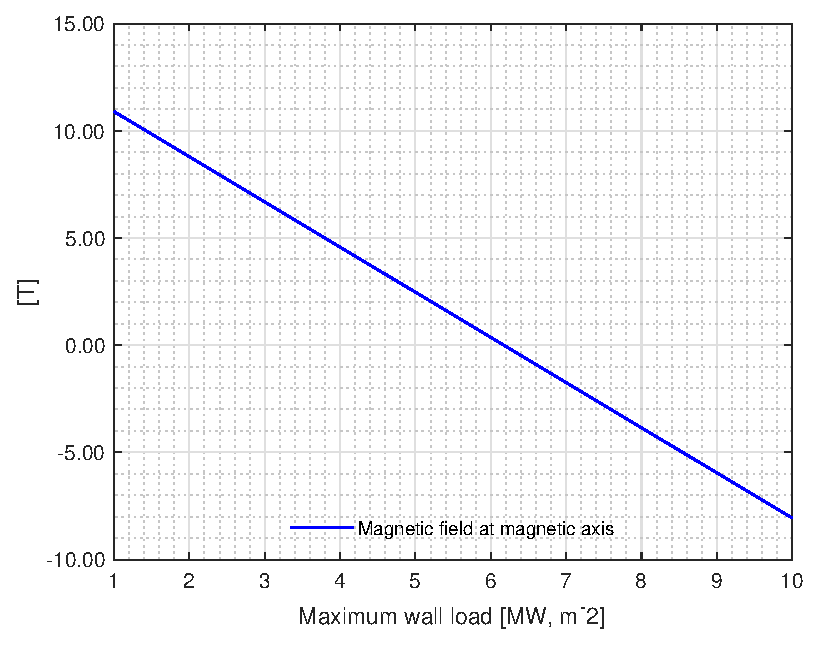
\includegraphics[width=\textwidth]{MatlabFigures/PW/f7.eps}
	\end{subfigure}
	~
	\begin{subfigure}[h!]{.45\textwidth}
		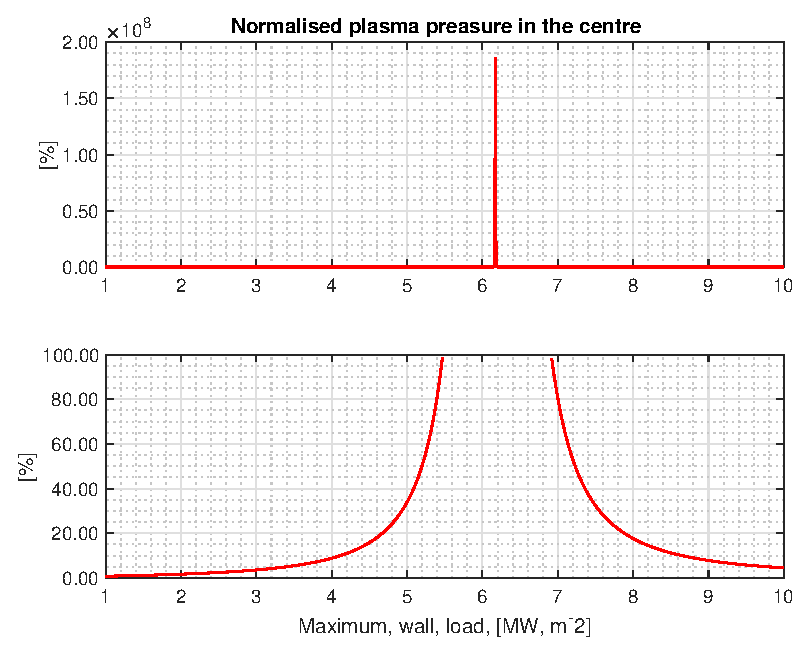
\includegraphics[width=\textwidth]{MatlabFigures/PW/f8.eps}
	\end{subfigure}
\end{figure}
\begin{figure}[H]
	\centering
	\begin{subfigure}[h!]{.45\textwidth}
		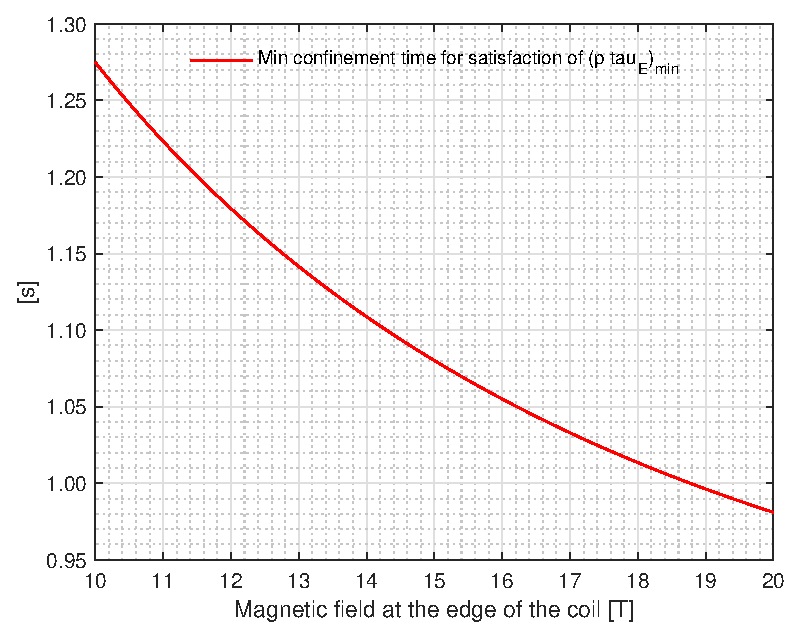
\includegraphics[width=\textwidth]{MatlabFigures/Bmax/f1.eps}
	\end{subfigure}
	~
	\begin{subfigure}[h!]{.45\textwidth}
		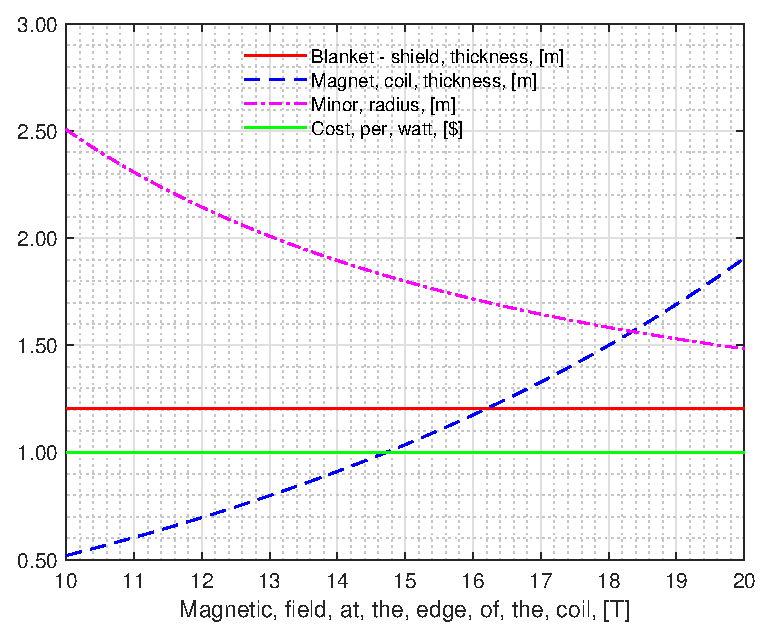
\includegraphics[width=\textwidth]{MatlabFigures/Bmax/f2.eps}
	\end{subfigure}

	\begin{subfigure}[h!]{.45\textwidth}
		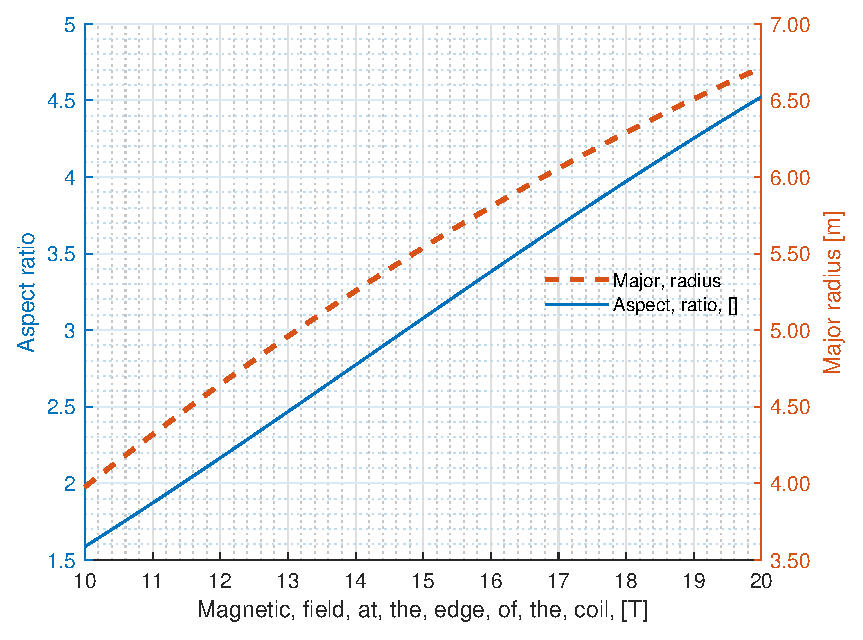
\includegraphics[width=\textwidth]{MatlabFigures/Bmax/f3.eps}
	\end{subfigure}
	~
	\begin{subfigure}[h!]{.45\textwidth}
		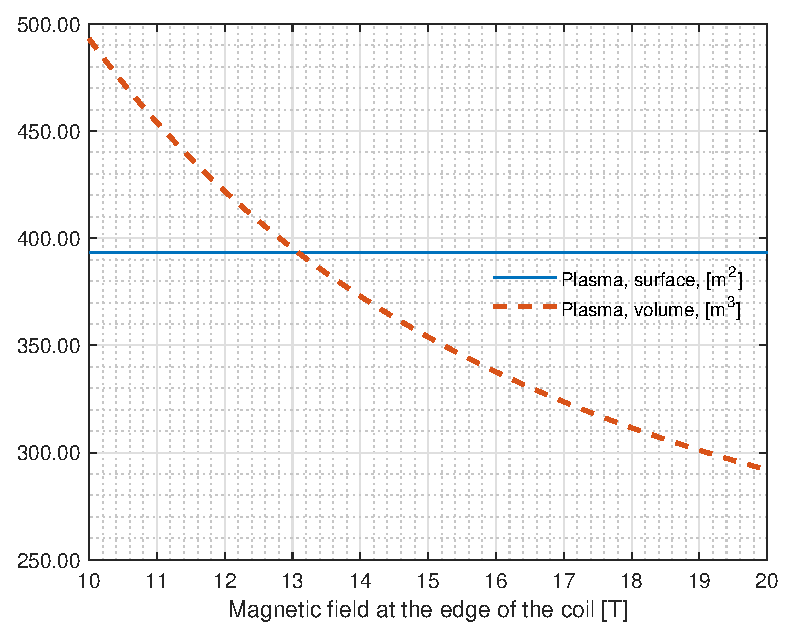
\includegraphics[width=\textwidth]{MatlabFigures/Bmax/f4.eps}
	\end{subfigure}

	\begin{subfigure}[h!]{.45\textwidth}
		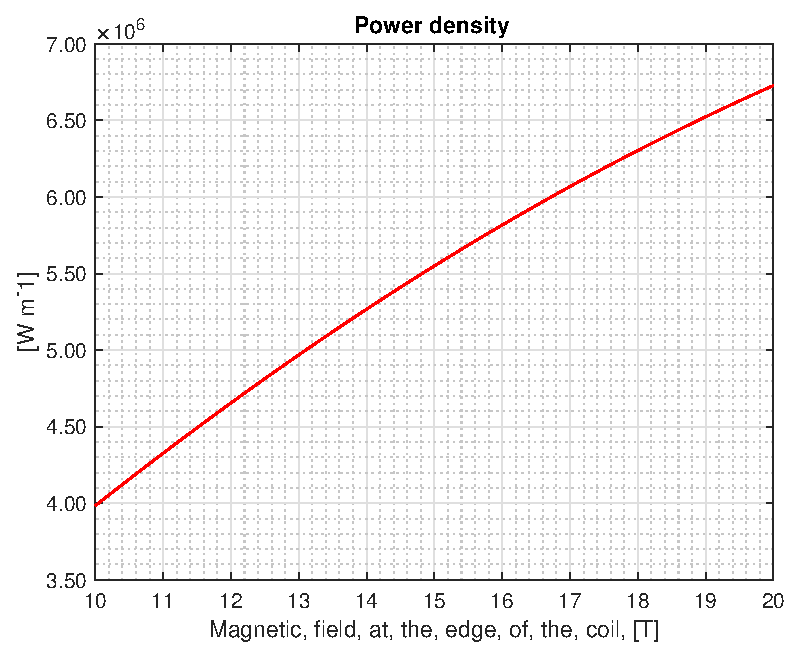
\includegraphics[width=\textwidth]{MatlabFigures/Bmax/f5.eps}
	\end{subfigure}
	~
	\begin{subfigure}[h!]{.45\textwidth}
		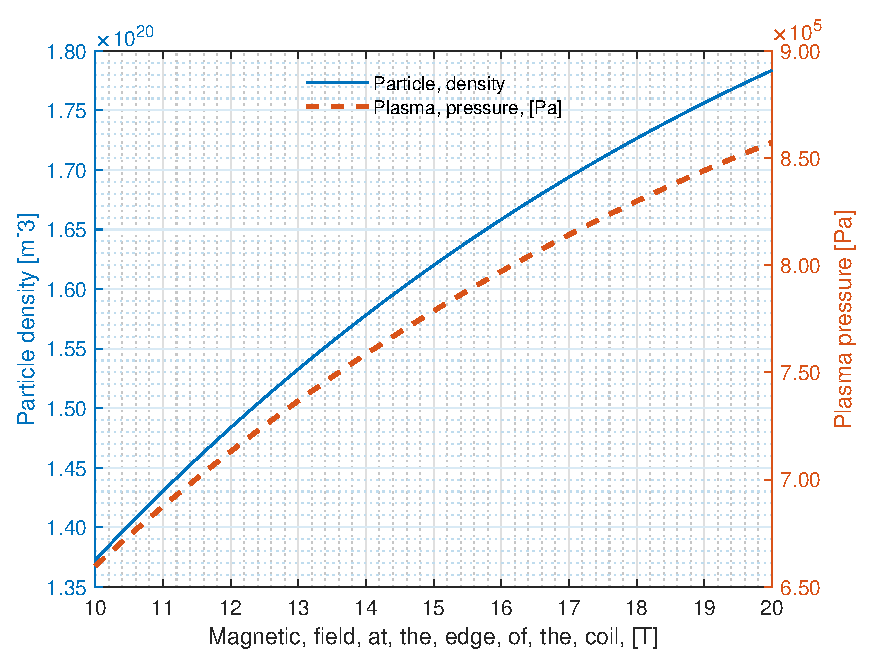
\includegraphics[width=\textwidth]{MatlabFigures/Bmax/f6.eps}
	\end{subfigure}

	\begin{subfigure}[h!]{.45\textwidth}
		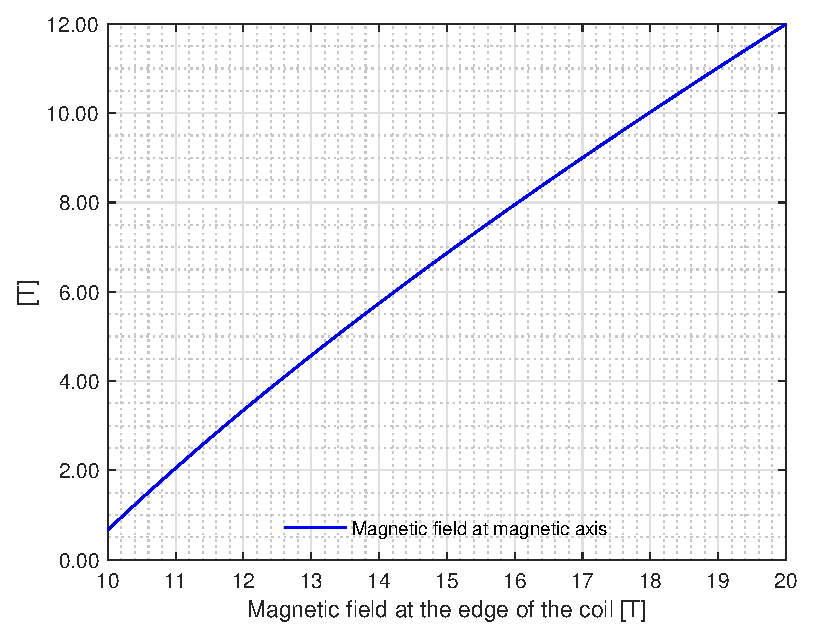
\includegraphics[width=\textwidth]{MatlabFigures/Bmax/f7.eps}
	\end{subfigure}
	~
	\begin{subfigure}[h!]{.45\textwidth}
		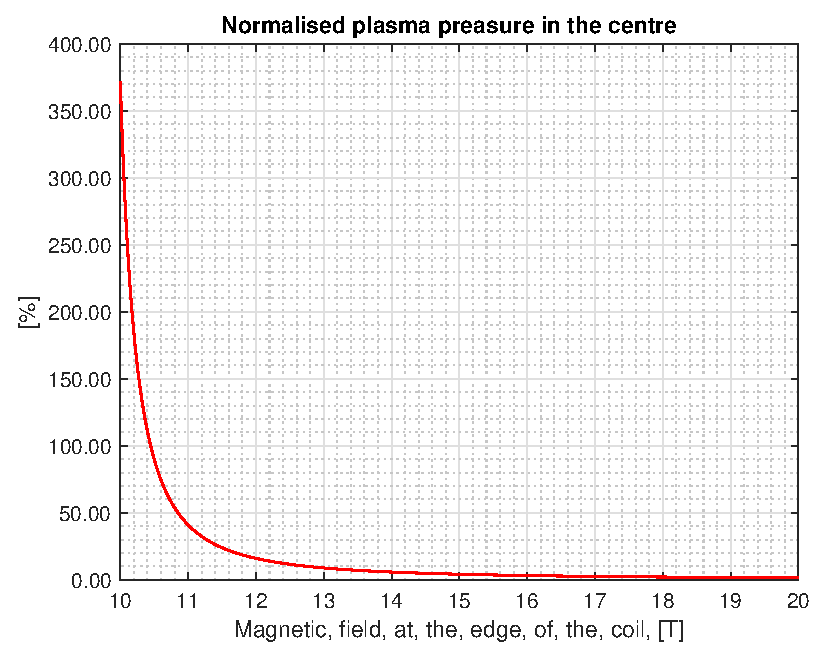
\includegraphics[width=\textwidth]{MatlabFigures/Bmax/f8.eps}
	\end{subfigure}
\end{figure}
\begin{figure}[H]
	\centering
	\begin{subfigure}[h!]{.45\textwidth}
		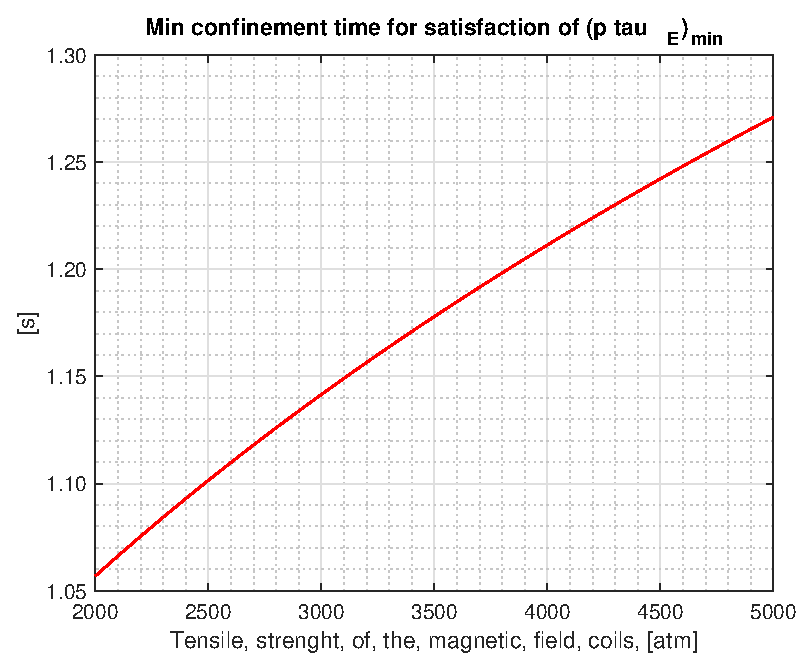
\includegraphics[width=\textwidth]{MatlabFigures/sigmamax/f1.eps}
	\end{subfigure}
	~
	\begin{subfigure}[h!]{.45\textwidth}
		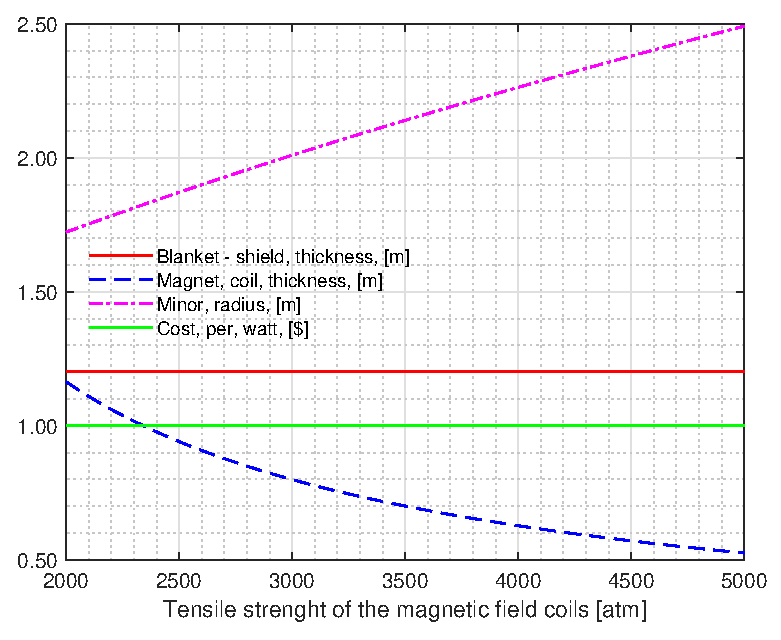
\includegraphics[width=\textwidth]{MatlabFigures/sigmamax/f2.eps}
	\end{subfigure}

	\begin{subfigure}[h!]{.45\textwidth}
		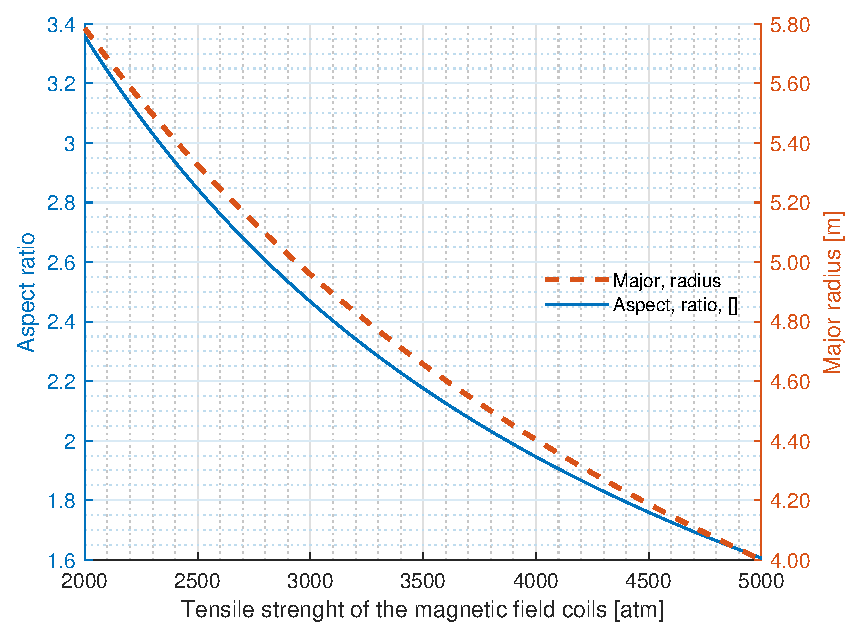
\includegraphics[width=\textwidth]{MatlabFigures/sigmamax/f3.eps}
	\end{subfigure}
	~
	\begin{subfigure}[h!]{.45\textwidth}
		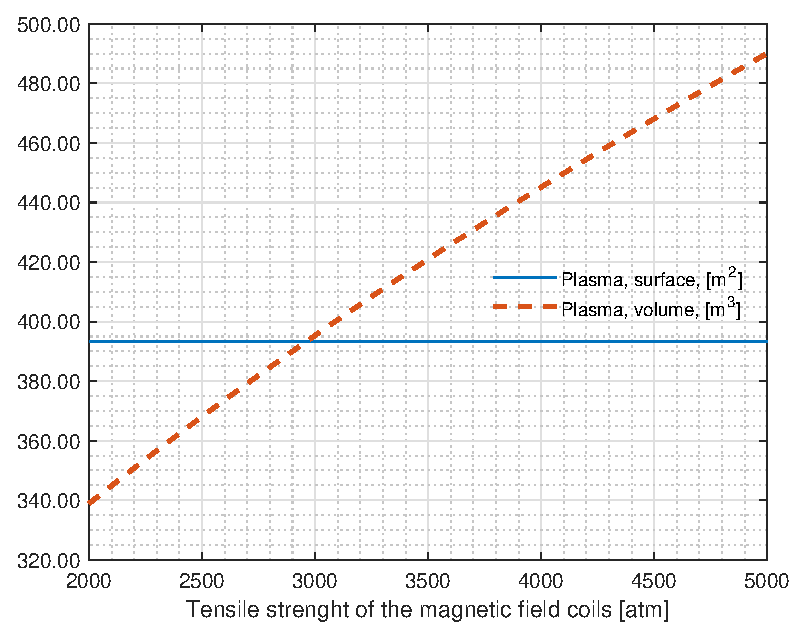
\includegraphics[width=\textwidth]{MatlabFigures/sigmamax/f4.eps}
	\end{subfigure}

	\begin{subfigure}[h!]{.45\textwidth}
		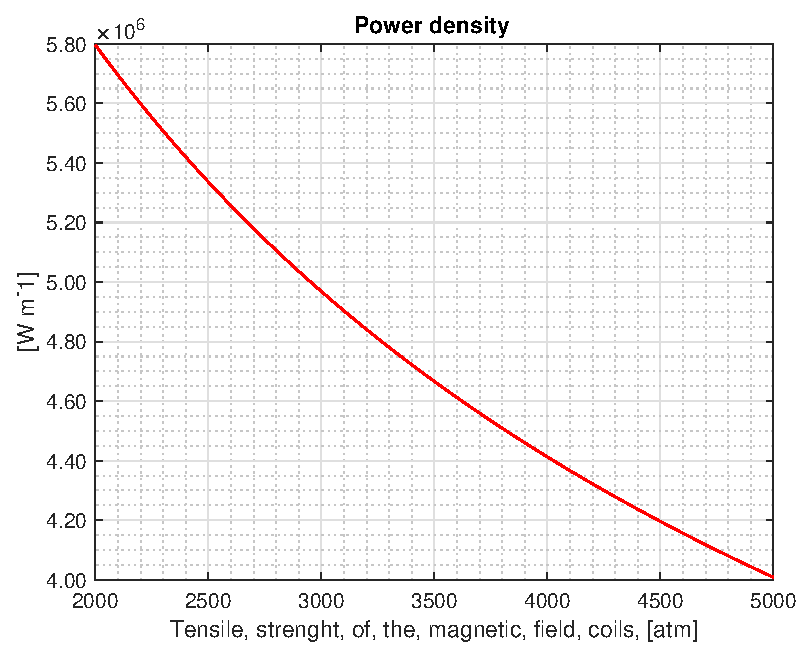
\includegraphics[width=\textwidth]{MatlabFigures/sigmamax/f5.eps}
	\end{subfigure}
	~
	\begin{subfigure}[h!]{.45\textwidth}
		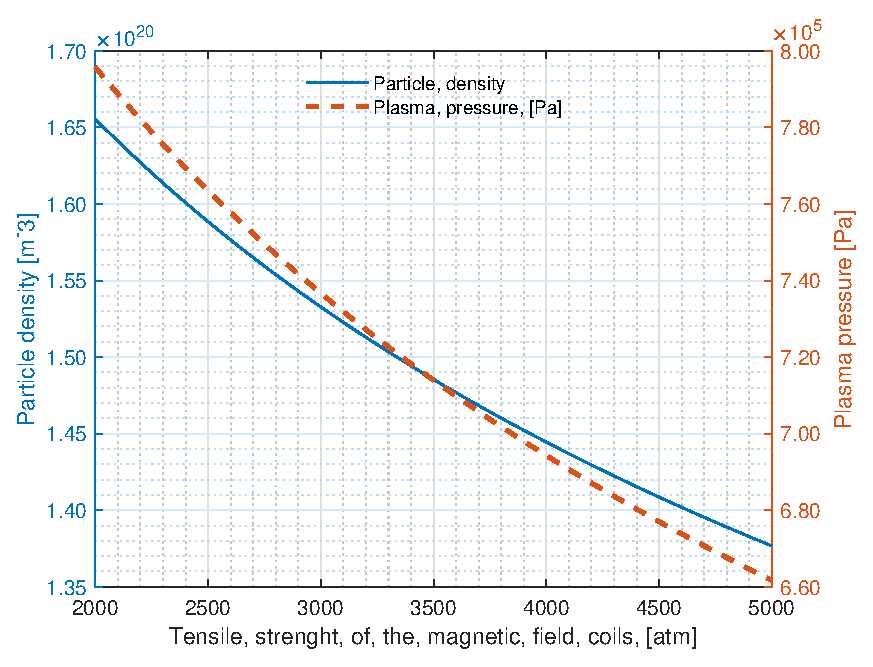
\includegraphics[width=\textwidth]{MatlabFigures/sigmamax/f6.eps}
	\end{subfigure}

	\begin{subfigure}[h!]{.45\textwidth}
		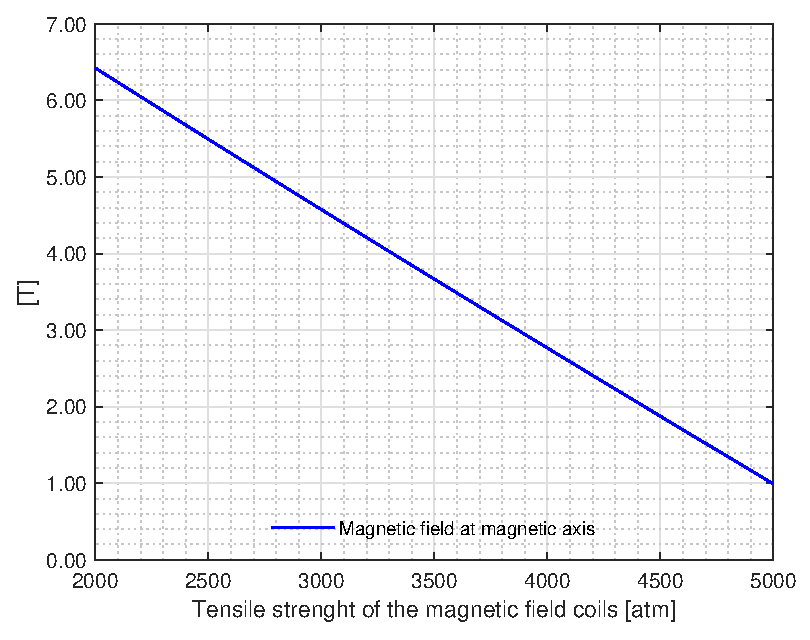
\includegraphics[width=\textwidth]{MatlabFigures/sigmamax/f7.eps}
	\end{subfigure}
	~
	\begin{subfigure}[h!]{.45\textwidth}
		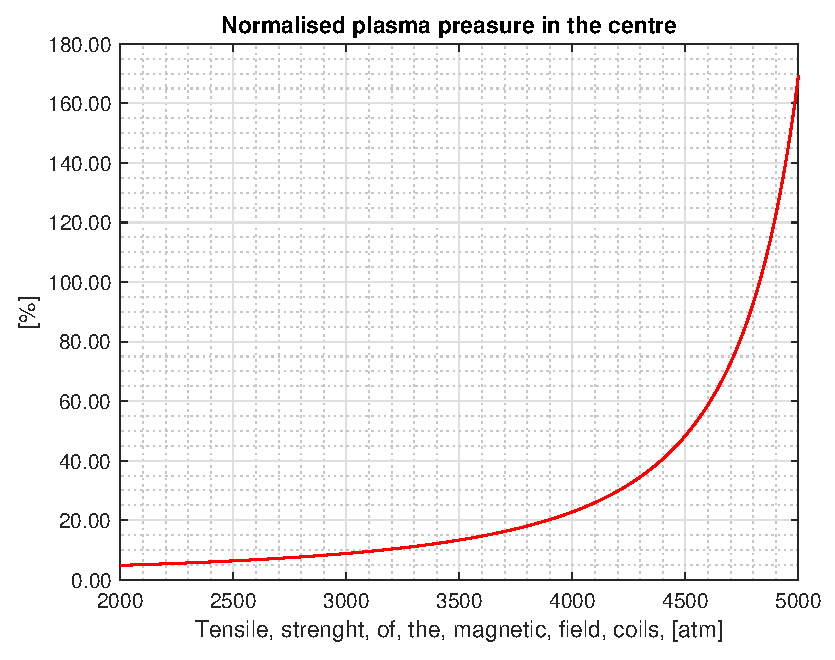
\includegraphics[width=\textwidth]{MatlabFigures/sigmamax/f8.eps}
	\end{subfigure}

\end{figure}
\newpage
\section{interferometer.m}\label{inter}
\inputminted[bgcolor=Black,linenos=true]{matlab}{Listings/interferometer.m}
\section{PhaseShiftDensity.m}
\inputminted[bgcolor=Black,linenos=true]{matlab}{Listings/PhaseShiftDensity.m}\label{PSD}

\end{document}
